\documentclass{amsart}
\usepackage{graphicx}
\graphicspath{{./}}
\usepackage{hyperref}
\usepackage{csvsimple}
\usepackage{longtable}
\usepackage{epigraph}
\title{Universal Morals Excluding Modern Sex Before Marriage, Homosexuality and Divorce}
\author{Zulfikar Moinuddin Ahmed}
\date{\today}
\begin{document}
\maketitle

I was examining the German values versus all other people and saw a great difference on Homosexuality, Sex Before Marriage, and Divorce.

I am refitting my model excluding these issues.

\section{Quality of Fit}

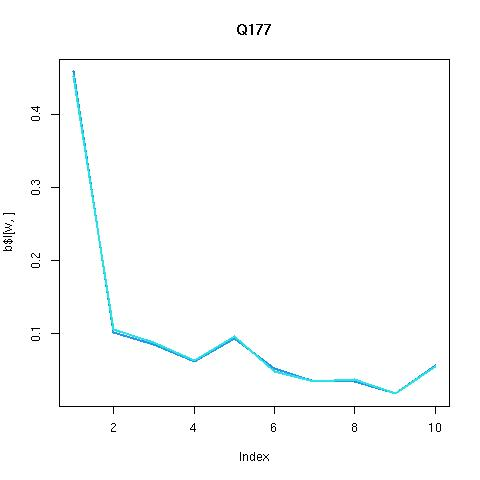
\includegraphics[scale=0.6]{fitQ177.jpeg}

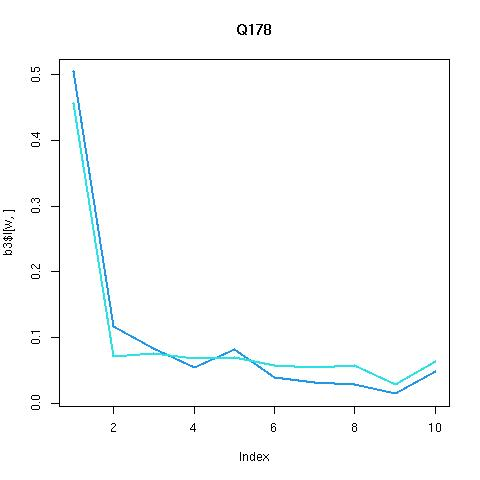
\includegraphics[scale=0.6]{fitQ178.jpeg}

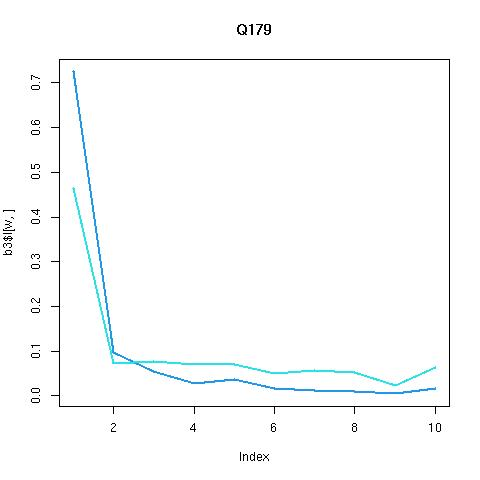
\includegraphics[scale=0.6]{fitQ179.jpeg}

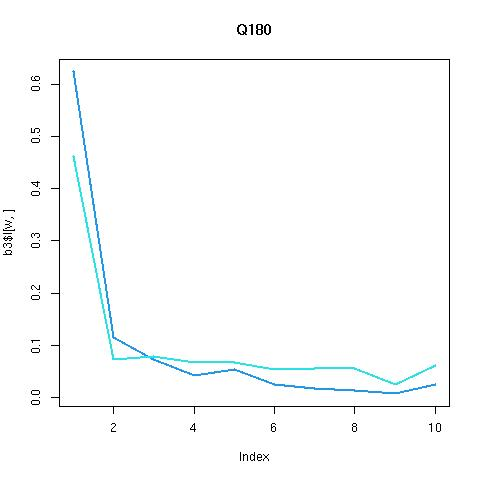
\includegraphics[scale=0.6]{fitQ180.jpeg}

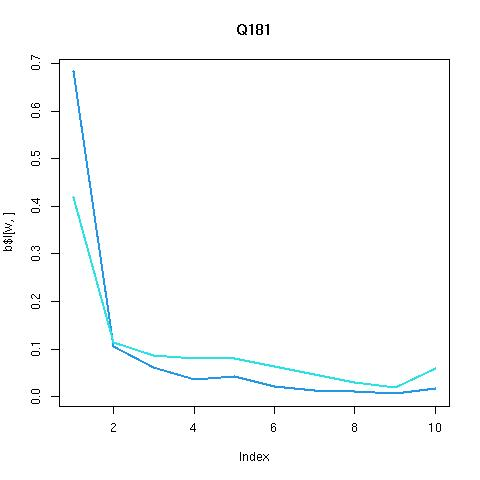
\includegraphics[scale=0.6]{fitQ181.jpeg}

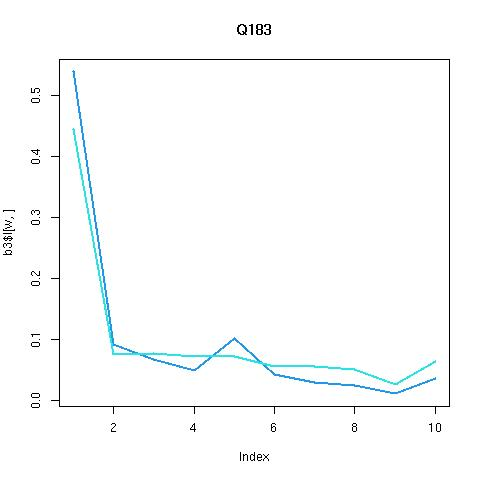
\includegraphics[scale=0.6]{fitQ183.jpeg}

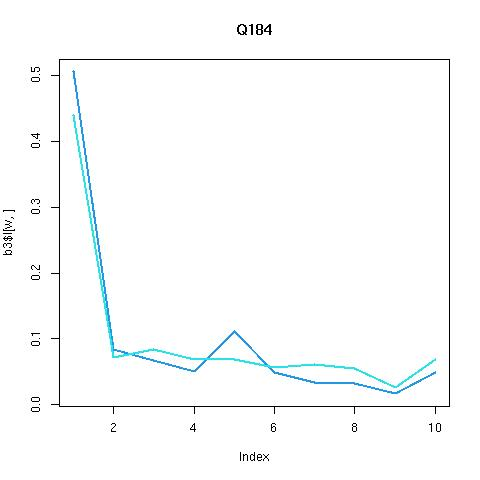
\includegraphics[scale=0.6]{fitQ184.jpeg}

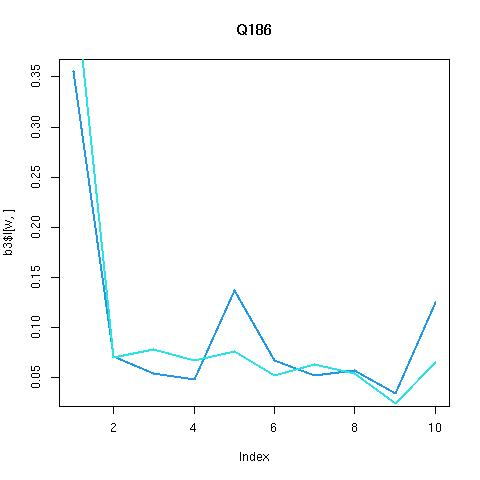
\includegraphics[scale=0.6]{fitQ186.jpeg}

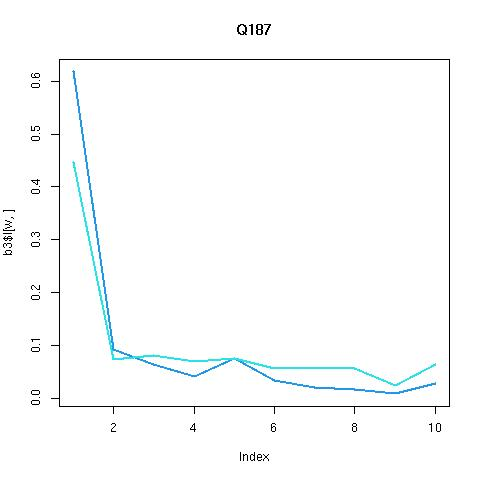
\includegraphics[scale=0.6]{fitQ187.jpeg}

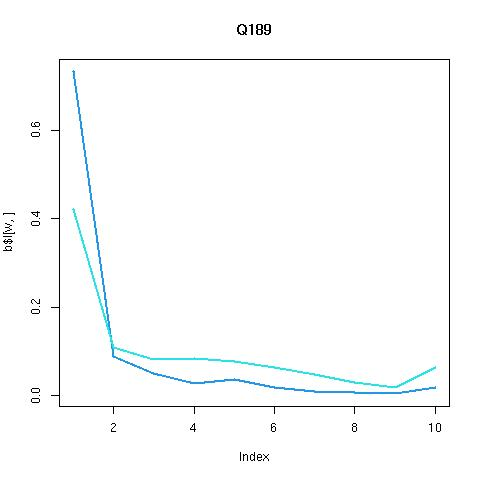
\includegraphics[scale=0.6]{fitQ189.jpeg}

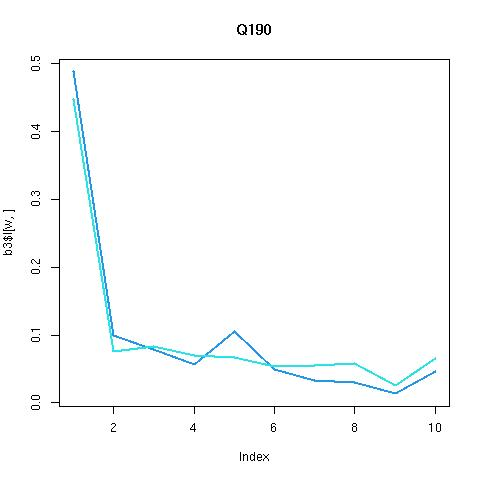
\includegraphics[scale=0.6]{fitQ190.jpeg}

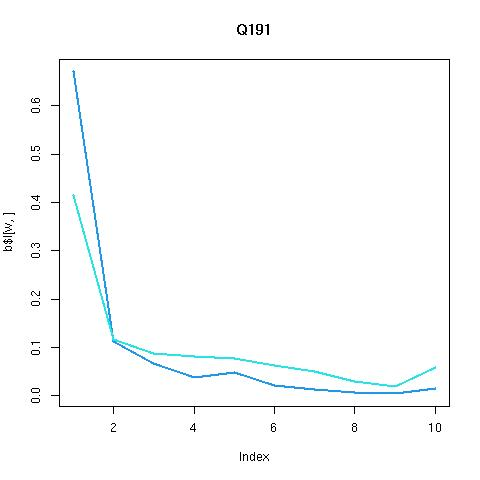
\includegraphics[scale=0.6]{fitQ191.jpeg}

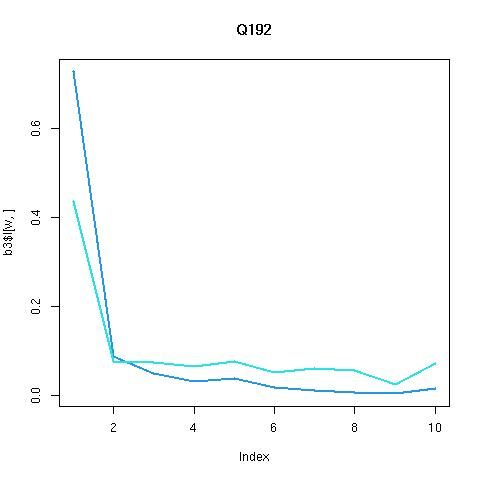
\includegraphics[scale=0.6]{fitQ192.jpeg}

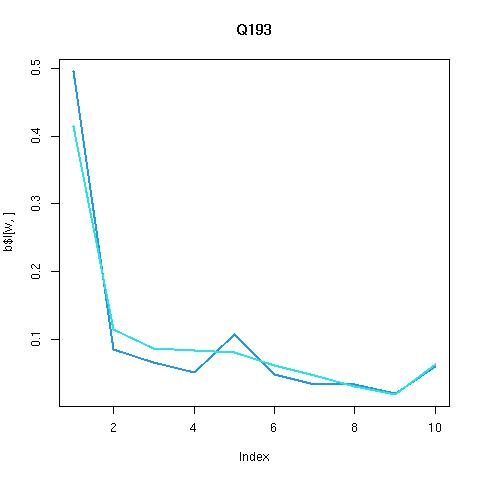
\includegraphics[scale=0.6]{fitQ193.jpeg}

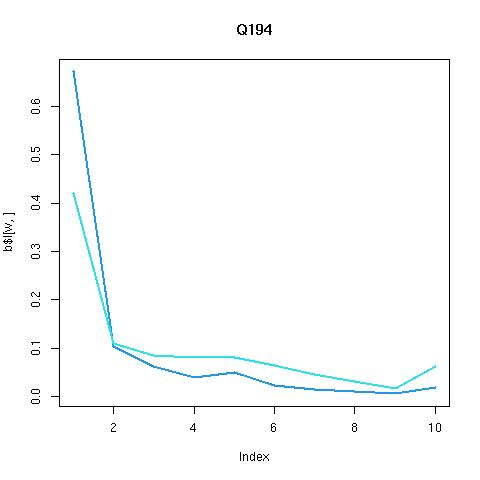
\includegraphics[scale=0.6]{fitQ194.jpeg}

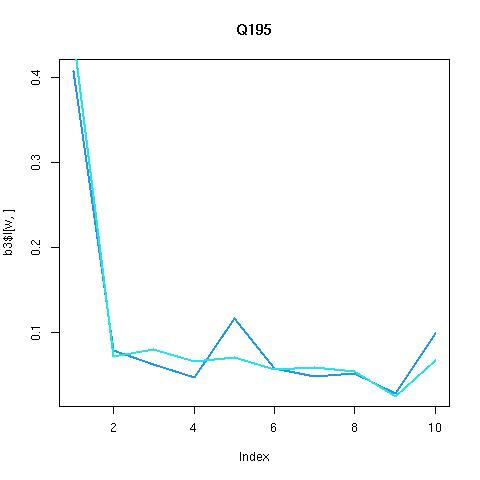
\includegraphics[scale=0.6]{fitQ195.jpeg}

There are all sorts of fine tuned mismatches but the shape is matching, the $L^2$ metric is 0.859 and $R^2$ proxy is around 0.89.  

We're matching 160 parameters with 55 parameters, which gives 2.9 parameters per line.  Fine features are not going to be detectable with 2.9 parameters per line so this is a fairly good success.

\section{Code}

\begin{verbatim}
# load data
wvs7<-readRDS("wvs7.rds")

# Create ethnicity table 
# by mapping various detailed
# country-based ethnicities to
# broader groups
library(haven)
# Problem is WVS Q290 has too many 
# gradations when we want to deal 
# with a few classes that can allow 
# us to overcome ethnic prejudices
ethnicities<-unique(as.character(as_factor(wvs7$Q290)))

reduced_ethnicities<-function(){
  mapeth<-rep("Other",length(ethnicities))
  mapeth[c(1,7,15,33,38,43,65,107,154,210,214)]<-"White"
  mapeth[c(3,223,222,51,52,53,54,55,56,45,39,36,11)]<-"Black"
  mapeth[c(6,13,19,20,21,22,67,70)]<-"Indian"
  mapeth[c(4,17,48,97,98,99,100)]<-"Arab"
  mapeth[c(5,14,16,62,63,64,68,72,73,74,75,76,77,
           78,79,80,81,82,83)]<-"East Asian"
  data.frame(key=ethnicities,val=mapeth)
}

ethnicity_map<-function( v ){
  emap<-reduced_ethnicities()
  w<-sapply(as.character(as_factor(v)),function(x) { out<-emap[which(emap$key==x),]$val; if(is.null(out)){out<-"Other"};return(out)})
  #print(head(w))
  #w<-append(w,"Other")
  as.factor(unlist(w))
}



polv<-na.omit(wvs7[,c("Q290",vars)])
polv$eth<-ethnicity_map(as_factor(polv$Q290))

# Fit P to distributions to Q177-Q195 in WVS 7
library(markovchain)

t10 <-1:10
nrm<-function(v)v/sum(v)

transitionMatrixFromPars<-function(x){
  P<-matrix(0,nrow=10,ncol=10)
  P[1,1]<-x[1]
  P[1:2,2]<-x[2:3]
  P[1:3,3]<-x[4:6]
  P[1:4,4]<-x[7:10]
  P[1:5,5]<-x[11:15]
  P[1:6,6]<-x[16:21]
  P[1:7,7]<-x[22:28]
  P[1:8,8]<-x[29:36]
  P[1:9,9]<-x[37:45]
  P[1:10,10]<-x[46:55]
  #symmetrize
  for (k in 2:10){
    P[k,1:k]<-P[1:k,k]
  }
  for (k in 1:10){
    P[k,]<-nrm(P[k,])
  }
  P
}

parsFromTransitionMatrix<-function(P){
  x<-c()
  for (k in 1:10){
    x<-append(x, P[1,1:k])
  }
  x
}

# We let x be the parameters of the subdiagonal
# of P in form appropriate for an optimiser
moral_markov_obj<-function( x ){
  
  P <- transitionMatrixFromPars( x )
  states <- as.character(1:10)
  mcVals = new("markovchain", 
               states = states,
               transitionMatrix = P,          
               name = "Vals")
  nvars<-length(vars)
  Imtx <- matrix( 0, nrow=nvars,ncol=10)
  Jmtx <- matrix( 0, nrow=nvars, ncol=10)
  I<-nrm(table(polv[,vars[1]]))
  Imtx[1,] <- I
  M<-10000
  Y1<-sample(1:10,M,replace=TRUE,prob=I)
  all.Y<-matrix(0,nrow=M,ncol=nvars)
  all.Y[,1]<-Y1
  for (kk in 1:M) {
    #print(kk)
    outs <- markovchainSequence(n = nvars-1, markovchain = mcVals, 
                                t0 = all.Y[kk,1], 
                                include.t0 = TRUE )
    all.Y[kk,1:nvars]<-outs  
  }

  for ( r in 1:nvars){
    iv<-nrm(table(polv[,vars[r]]))
    jv<-nrm(table(all.Y[,r]))
    ivn<-rep(0,10)
    jvn<-rep(0,10)
    for ( kc in 1:10 ){
      a<-iv[as.character(kc)]
      b<-jv[as.character(kc)]
      if (!is.null(a)){
          ivn[kc]<-a
      }
      if (!is.null(b)){
        jvn[kc]<-b
      }
        
    }
    Imtx[r,]<-ivn
    Jmtx[r,]<-jvn
  }

  print('calculating l2 distance')  
  l2.dist <- 0
  l2.ldist <- 0
  sld.dist<-0
  rsq.proxy<-0
  hits<-0
  for (r in 1:nvars){
    d1<- norm(abs(Imtx[r,]),type="2")
    d2<- norm(abs(Jmtx[r,]),type="2")
    A <-log(Imtx[r,]+1e-6) - log(Jmtx[r,]+1e-6)
    d <- norm( Imtx[r,] - Jmtx[r,], type="2")
    suplogd <-norm( as.matrix(A), type="I")
    dl <- suplogd + 10*d
    #print(paste("r=",r,"d1=",d1,"d2=",d2,"d=",d))
    if (!is.na(d)){
      hits<-hits+1
      sld.dist <- sld.dist + suplogd
      l2.ldist <- l2.ldist + dl
      l2.dist <- l2.dist + d^2
      rsqp <- 1 - d^2/d1^2
      rsq.proxy <- rsq.proxy + rsqp
    }
  }
  #l2.ldist<-l2.ldist
  print(paste("sld=",sld.dist))
  print(paste("l2 log dist=",l2.ldist))
  l2.dist<-sqrt(l2.dist)
  print(paste("l2 dist=",l2.dist))
  
  rsq.proxy <- rsq.proxy/hits
  print(paste('rsq.proxy=',rsq.proxy))
  l2.ldist
}




library(nloptr)
# Get an init value
lambda <- 0.52
p11 <- 0.6
P <- matrix(0,nrow = 10, ncol=10)
P[1,1] = p11
for (k in 2:10){
  for (r in 1:k){
    P[k,r] <- exp(-lambda*(k+r))*p11
    P[r,k] <- P[k,r]
  }
}
for ( r in 1:10){
  P[r,]<-P[r,]/sum(P[r,])
}
P0<-P

x0<-parsFromTransitionMatrix(P0)
xlen <- length(x0)
l0 <- rep(0,xlen)
u0 <- rep(1,xlen)

eval_g0<-function( x ){
  P1<-transitionMatrixFromPars(x)
  out<-0
  for (k in 1:10){
    out <- out + (sum(P1[k,]))^2-1.0
  }
  out
}

# Solve using NLOPT_LN_COBYLA without gradient information
res2 <- nloptr( x0=x0,
                eval_f=moral_markov_obj,
                lb = l0,
                ub = u0,
                opts = list("algorithm"="NLOPT_LN_NELDERMEAD",
                            "xtol_rel"=1.0e-6,
                            "maxeval"=5000,
                            "print_level"=1))
print( res2 )
\end{verbatim}

The code is self-explanatory.  I use the markovchain package, and the markovchainSequence function to simulate.

\end{document}
